
\begin{figure*}[t]
  \centering
  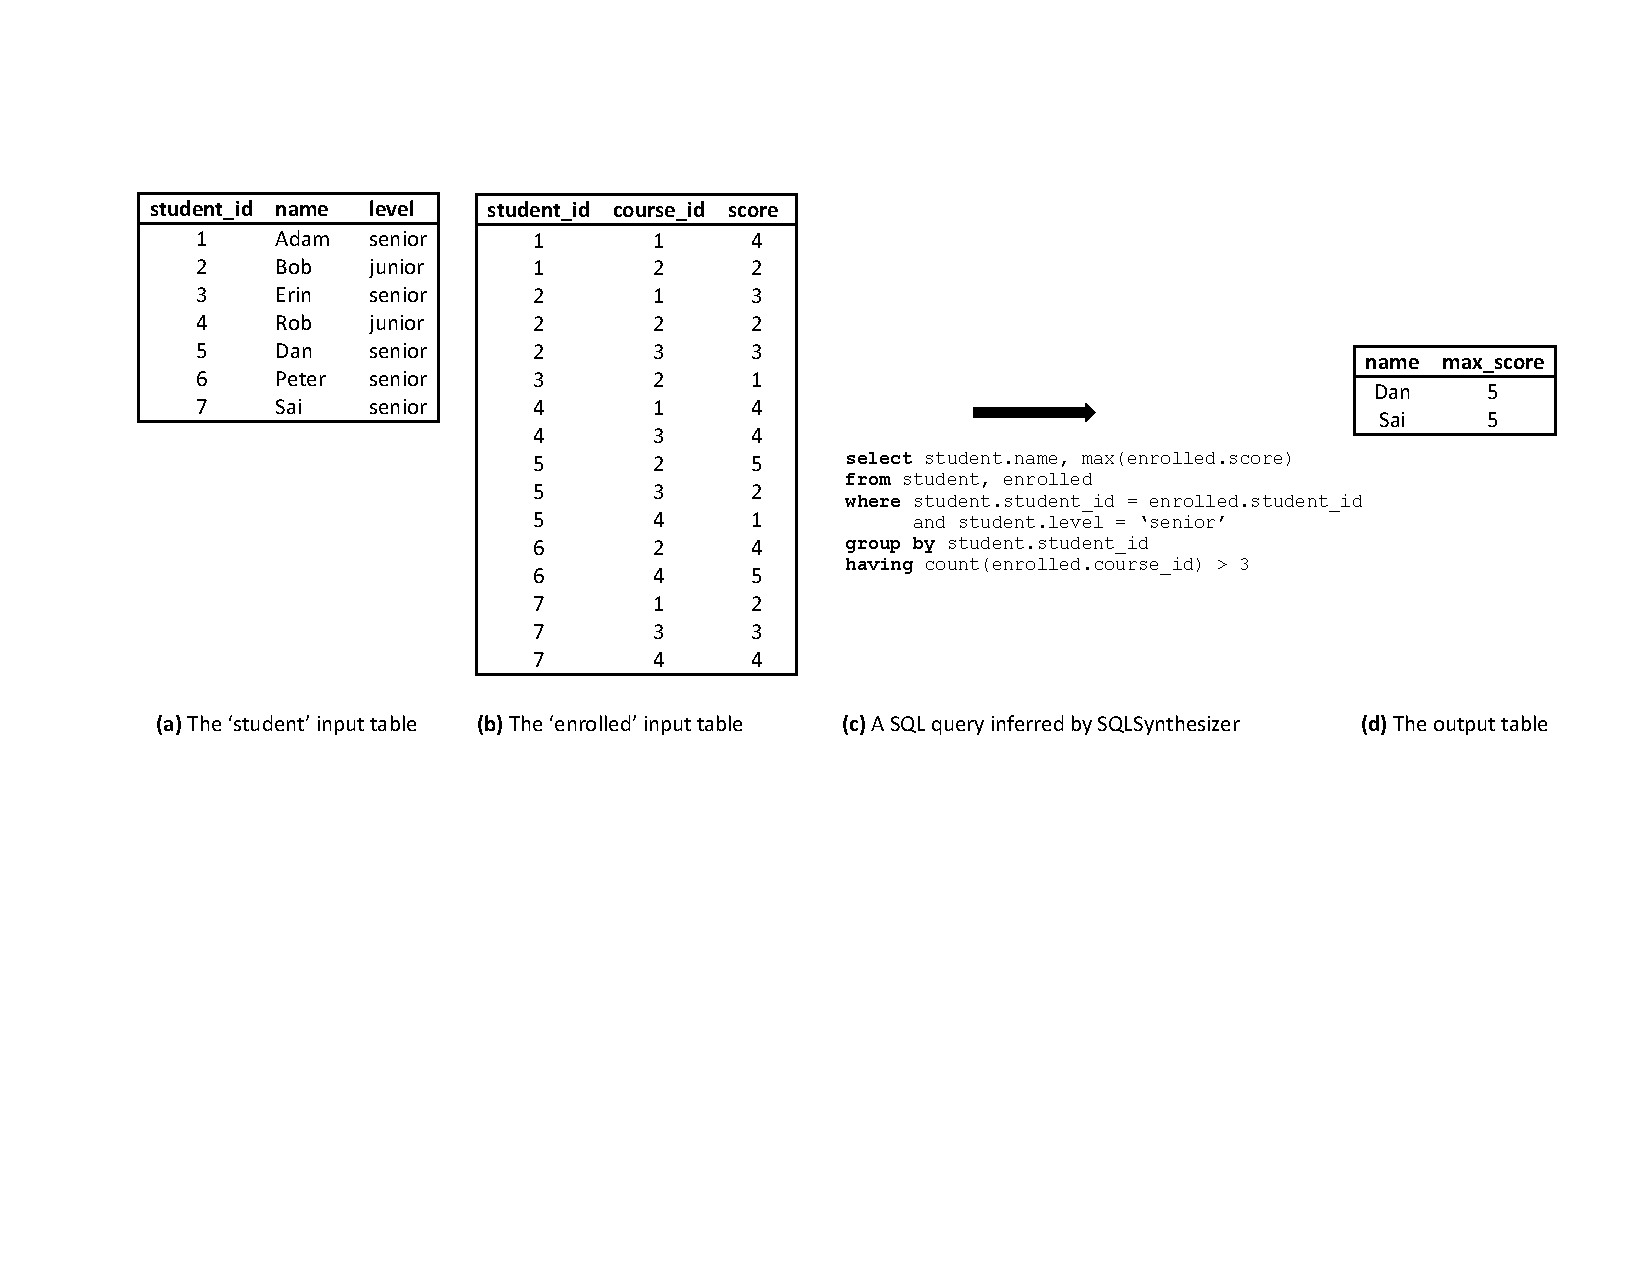
\includegraphics[scale=0.70]{motivating}
  \vspace*{-1.0ex}\caption {{\label{fig:motivating}
  Example input-output tables and the SQL query sythensized by
  \ourtool. In this example, users provide \ourtool with
  two input tables (shown in (a)) and an output table (shown in (c));
  \ourtool automatically infers a SQL query (shown in (b)) that
  transforms the two input tables into the output table.
}}
\end{figure*}

\section{Illustrating Example}
\label{sec:example}

We use a SQL exercise from a classic database textbook~\cite{cowbook} (Chapter 5, Exercise \todo{xx})
as an example to illustrate the use of \ourtool.

\begin{quote}
\textit{Find out the name and max score of the students whose
level is senior and enrolled in more than 3 courses.}\footnote{
As described in the textbook, there is a \CodeIn{student} table
having two columns: \CodeIn{student\_id} and \CodeIn{nameA}, and
a \CodeIn{enrolled} table having three columns:
\CodeIn{student\_id}, \CodeIn{course\_id}, and \CodeIn{score}.}
\end{quote}


Although the problem description is quite clear and
most end-users have a clear idea of what the desirable
query should do, they \todo{still have difficult ...}

As an alternative solution, end-users can use \ourtool
to solve this peroblem. As depicted in Figure~\ref{fig:motivating},
a user provides \ourtool two input tables and one expected
output table. \ourtool automatically inferred the desirable
SQL query (Figure~\ref{fig:motivating}(b)) to produce the output from the input tables.


The synthesized query by \ourtool first joins the student, then ... \todo{project, and
aggregation}


\todo{add the following justification}
To the best of our knowledge, none of the
existing techniques can do ...
